\section{Formula student driverless}

Revolve NTNU is a team competing in various competitions around Europe in what is known as Formula Student. Formula Student is often referred to as the worlds largest engineering competition for students. It consists of several competitions spread around the globe, one of the most influential of which is \gls{FSG}. Over 300 students in 66 teams from 8 different countries competed at \gls{FSG} 2018. Revolve NTNU team 19 is seen in figure \ref{Fig:Team19}, along with the two cars that are to be used this year.

\begin{figure}
    \centering
    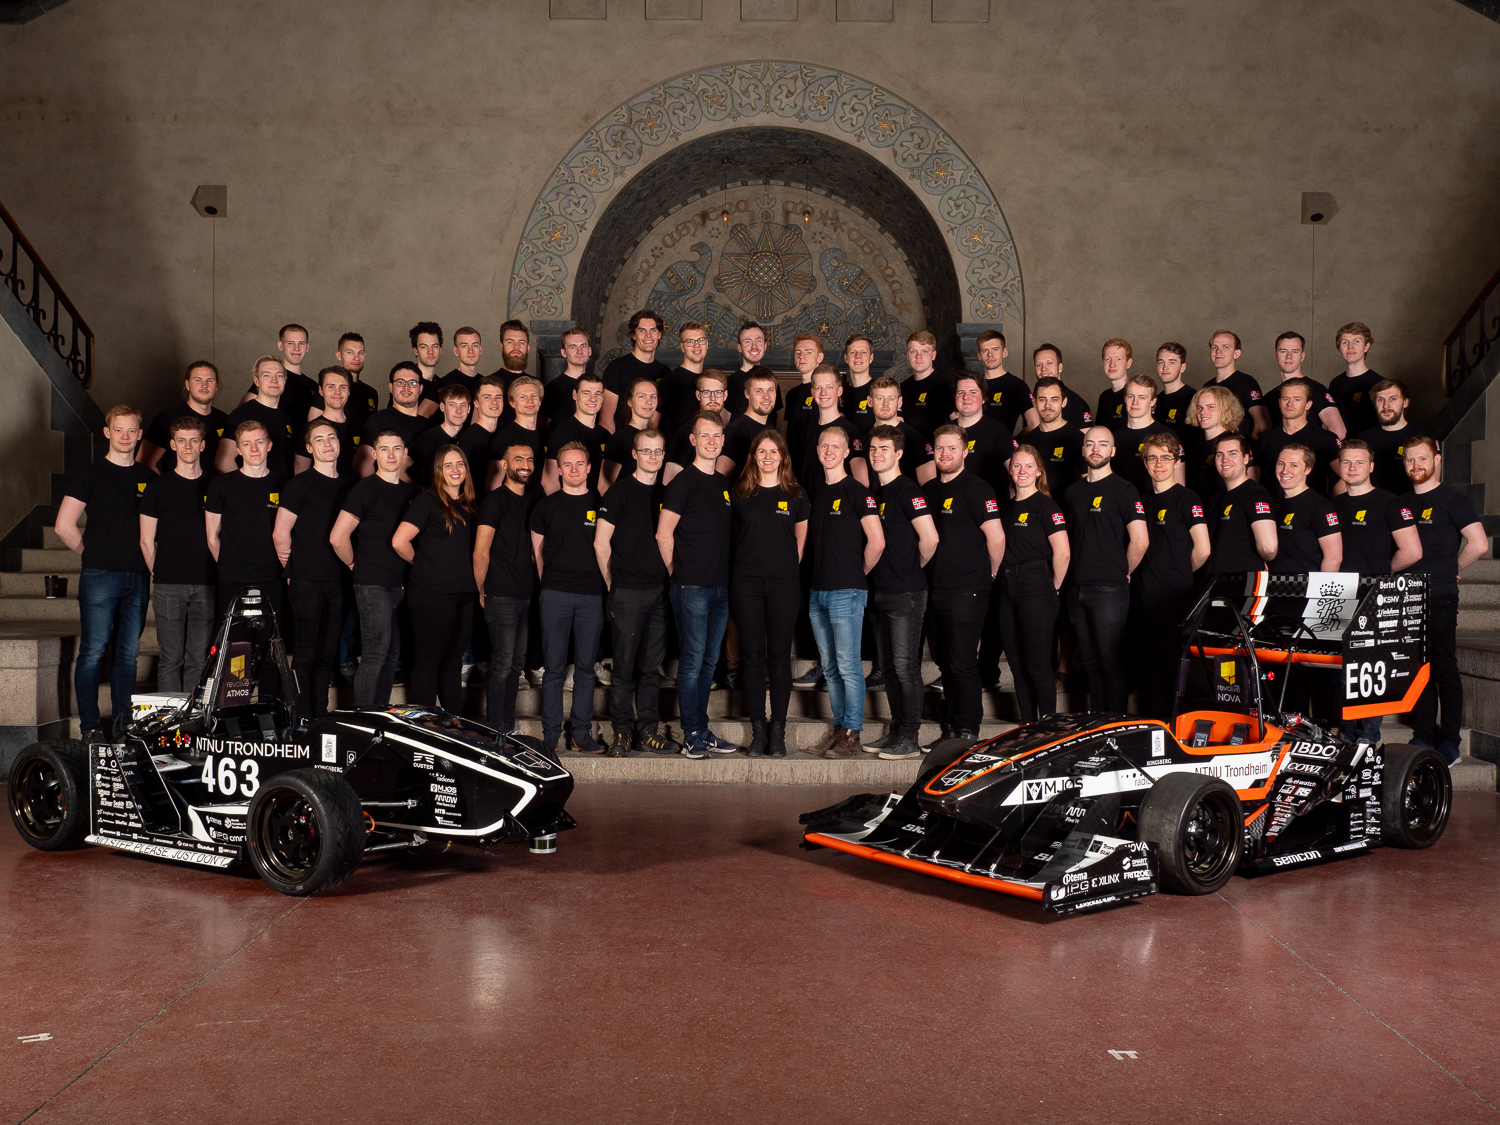
\includegraphics[width=\linewidth]{0_Images/2_Introduction/team19.jpg}
    \caption[Team 19, Revolve NTNU]{Team 19, Revolve NTNU. The car on the left is Atmos, this years driverless car, while the car on the right is the new electrical car, Nova.}
    \label{Fig:Team19}
\end{figure}

Each competition follows more or less the same recipe. First the car has to get through the very strict scrutineering. This means it has to follow all the safety and quality guidelines stated in the rules of the competition. Most teams do not get through this. If the car passes it then goes on to compete in one of three classes: combustion, electric or driverless. 

Competing implies both static and dynamic events, where the static events are focused on cost, documentation of the engineering process, and so on. The dynamic events for the combustion and electric class encompasses showing how energy efficient the car is, how well it accelerates, corners, etc. 

The driverless class is a rather new one, having been introduced at \gls{FSG} in 2017. Revolve NTNU had its first driverless team in 2018. Each driverless car is tested in four dynamic events: Acceleration, Skidpad, Autocross and Trackdrive. Each of the events are to be done without a driver in the car and without signals being sent to the car from the team in any way. In all events the goal is to drive as fast as possible without knocking any delimiters. The delimiters are blue cones on the left side and yellow cones on the right and knocking a delimiter gives a time penalty.

The acceleration event is just a 75 meter straight path, very much akin to a drag race. Skidpad has the car driving in a figure eight pattern, taking two loops on each circle, only being timed on the second run of each circle. Autocross is one round of an unknown track, where it is not allowed to do any mapping before starting the event. Trackdrive is the same as autocross, only now driving 10 rounds. 

Each event therefore requires somewhat different approaches. What is however constant is the need for good state estimation, detection, localisation and mapping. This allows the the car to drive fast without hitting any delimiters.